\section{Resultados}\label{sec:resultados}

\begin{frame}{Análisis de la presión}
    \begin{minipage}{0.45\textwidth}
        \begin{block}{Parámetros variables}
            \begin{itemize}
                \item $v_0 = 1\ m/s$
                \item $N = 200$
                \item $I = 1$
                \item $T = 20\ s$
            \end{itemize}
        \end{block}
    \end{minipage}
    \hfill
    \begin{minipage}{0.45\textwidth}
        \begin{figure}[H]
            \centering
            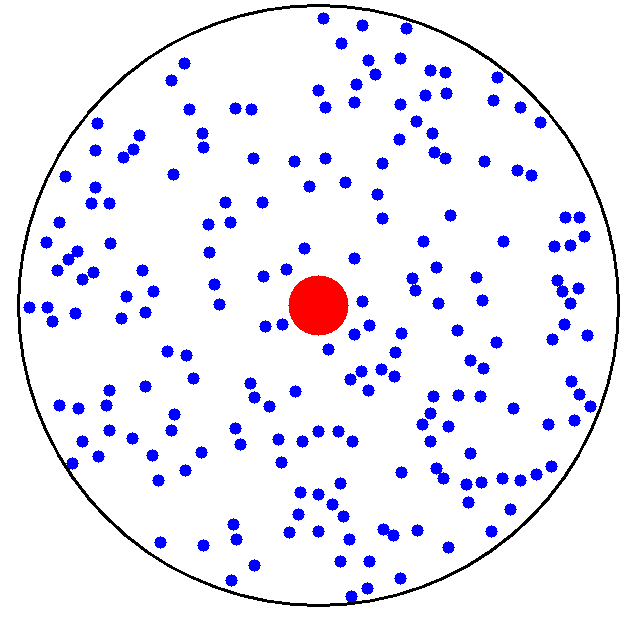
\includegraphics[width=0.8\textwidth]{pic/1.1/animation_1}
            \label{fig:av1}
        \end{figure}
        \tiny{\href{https://youtu.be/HJ0c-XNuGG8}{https://youtu.be/HJ0c-XNuGG8}}
    \end{minipage}
\end{frame}


\begin{frame}{Análisis de la presión}
    \begin{minipage}{0.8\textwidth}
        \begin{figure}[H]
            \centering
            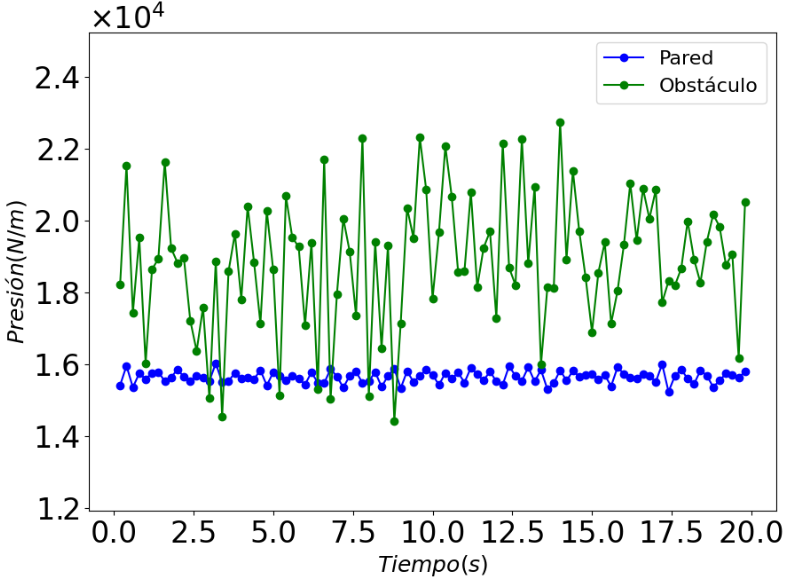
\includegraphics[width=0.85\textwidth]{pic/1.1/v1}
            \label{fig:tempvstime}
        \end{figure}
    \end{minipage}
    \hfill
    \begin{minipage}{0.15\textwidth}
        $v_0 = 1\ m/s$
    \end{minipage}
\end{frame}

\begin{frame}{Análisis de la presión}
    \begin{minipage}{0.75\textwidth}
        \begin{figure}[H]
            \centering
            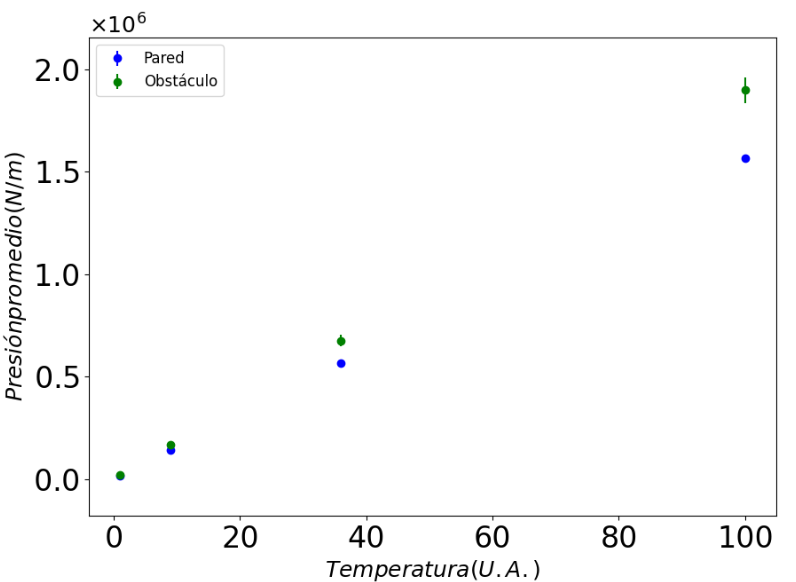
\includegraphics[width=0.9\textwidth]{pic/1.1/vstemp}
            \label{fig:tempvsTemp}
        \end{figure}
    \end{minipage}
    \hfill
    \begin{minipage}{0.2\textwidth}
        Valores iniciales de $v_0$:
        \begin{itemize}
            \item $1\ m/s$
            \item $3\ m/s$
            \item $6\ m/s$
            \item $10\ m/s$
        \end{itemize}
    \end{minipage}
\end{frame}



\begin{frame}{Colisión de Partículas Contra el Obstáculo}
    \begin{minipage}{0.25\textwidth}
        \begin{block}{Parámetros variables}
            \begin{itemize}
                \item $v_0 = 1\ m/s$
                \item $N = 300$
                \item $I = 10$
                \item $T = 5\ s$
            \end{itemize}
        \end{block}
    \end{minipage}
    \hfill
    \begin{minipage}{0.7\textwidth} % Adjust width to 70%
        \begin{figure}[H]
            \centering
            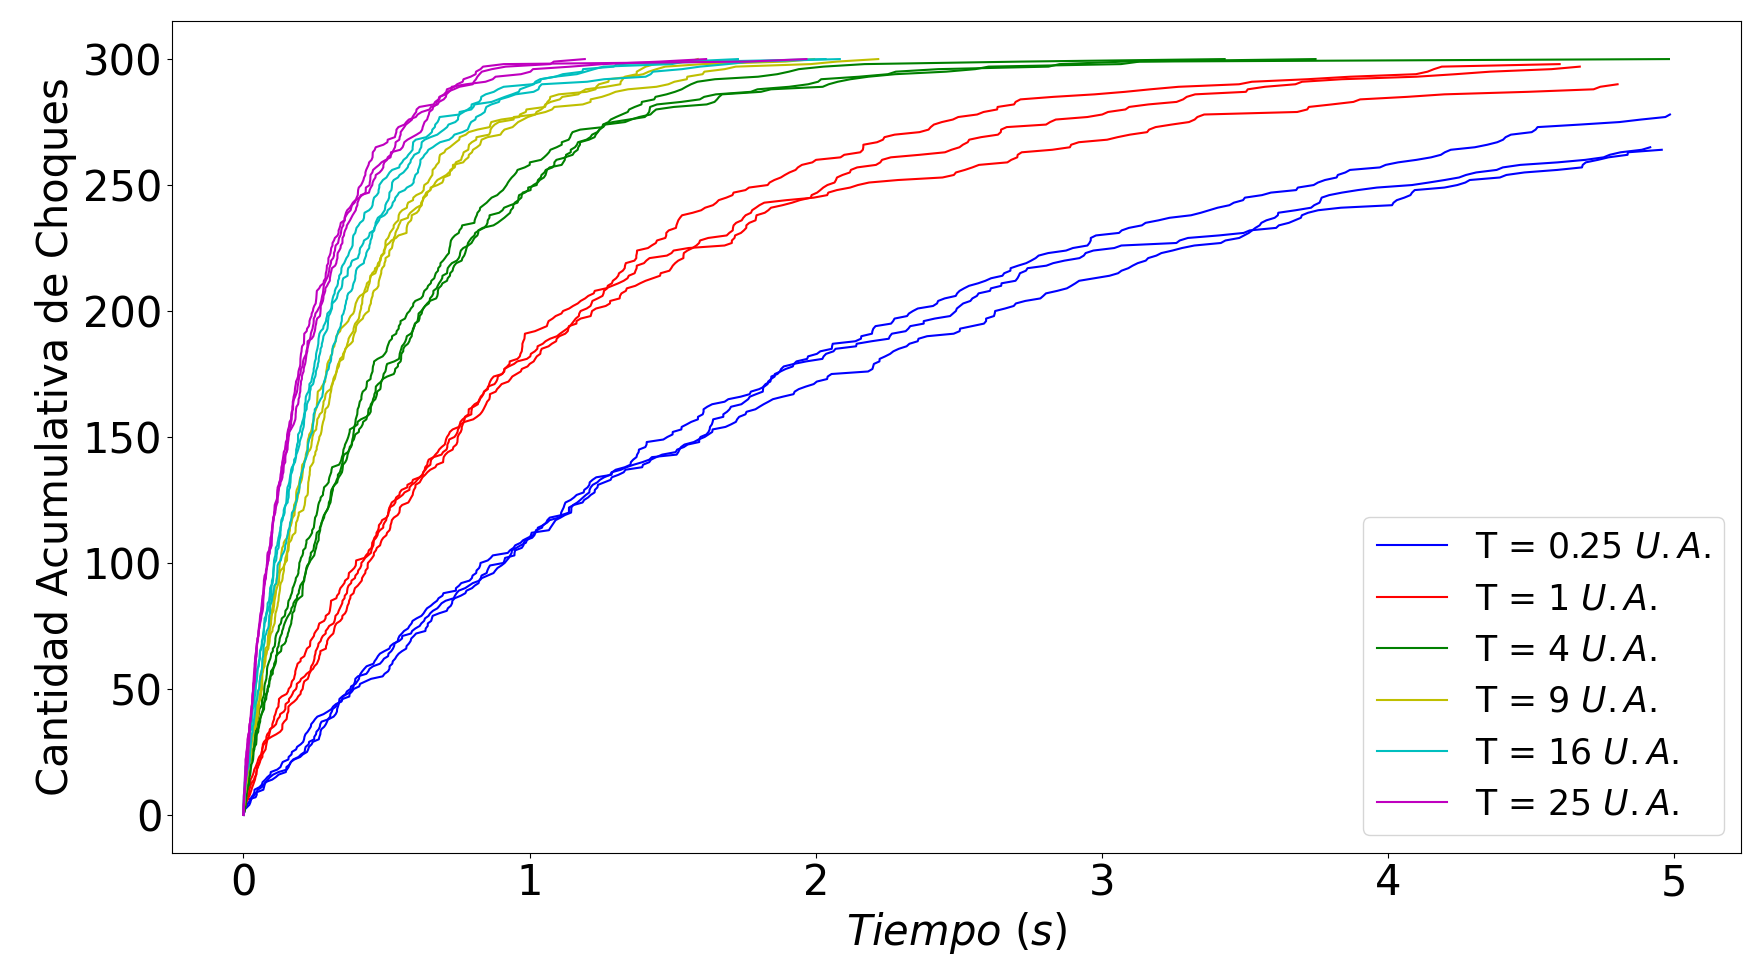
\includegraphics[width=0.9\textwidth]{pic/ejer3/a3Tiradas}
            \label{fig:ejer3:atiradas}
        \end{figure}
    \end{minipage}
\end{frame}

\begin{frame}{Colisión de Partículas Contra el Obstáculo}
    \begin{block}{Observable}
        Tiempo hasta que el 95\% de las partículas colisionó con el obstáculo en función de la Temperatura
    \end{block}

    \begin{figure}[H]
        \centering
        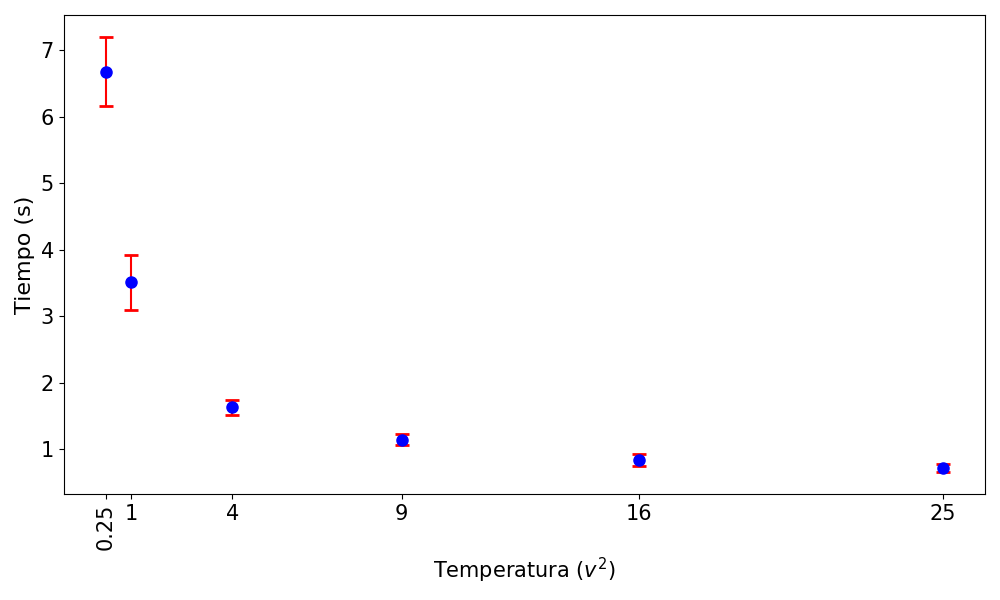
\includegraphics[width=0.6\textwidth]{pic/ejer3/aObs}
        \label{fig:ejer3:aobservable}
    \end{figure}

\end{frame}


\begin{frame}{Colisión de Partículas Contra el Obstáculo}

    \begin{block}{Colisiones}
        Ahora consideramos más de una colisión contra el obstáculo por partícula
    \end{block}

    \begin{minipage}{0.8\textwidth}
        \begin{block}{Parámetros variables}
            \begin{itemize}
                \item $v_0 = 1\ m/s$
                \item $N = 300$
                \item $I = 10$
                \item $T = 5\ s$
            \end{itemize}
        \end{block}
    \end{minipage}

\end{frame}


\begin{frame}{Colisión de Partículas Contra el Obstáculo}

    \begin{multicols}{2}
        {
            \begin{figure}[H]
                \centering
                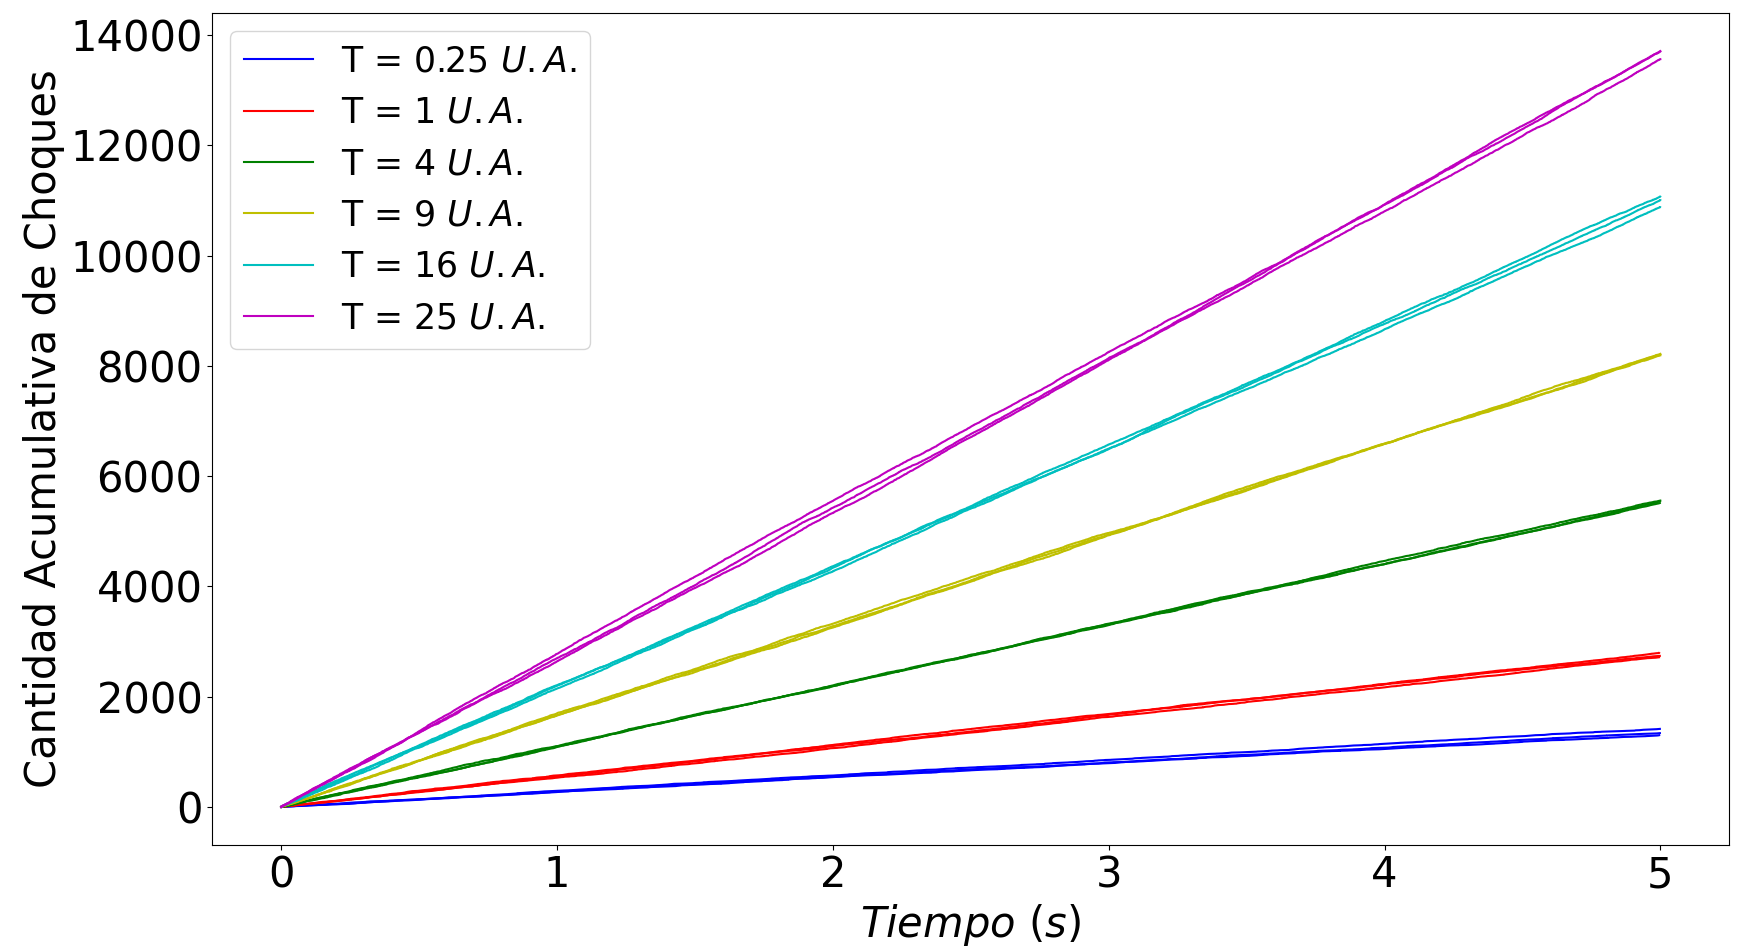
\includegraphics[width=0.8\linewidth]{pic/ejer3/b3Tiradas}
                \label{fig:ejer3:btiradas}
            \end{figure}
        }

        {
            \begin{figure}[H]
                \centering
                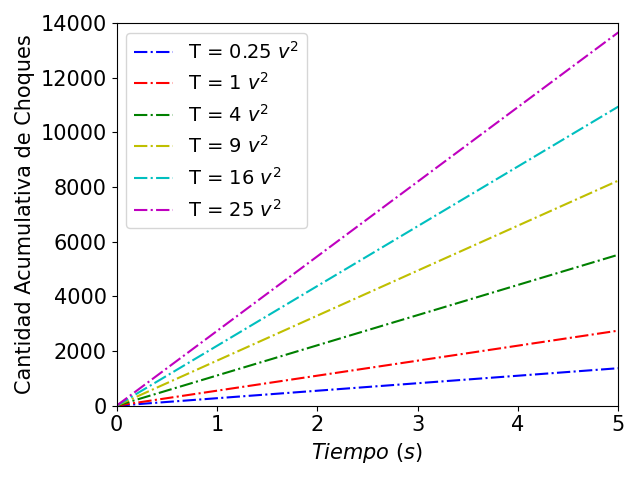
\includegraphics[width=0.8\linewidth]{pic/ejer3/bSoloSlopes}
                \label{fig:ejer3:bslopes}
            \end{figure}
        }
    \end{multicols}

\end{frame}


\begin{frame}{Colisión de Partículas Contra el Obstáculo}
    \begin{block}{Observable}
        Pendiente de la regresión lineal
    \end{block}

    \begin{figure}[H]
        \centering
        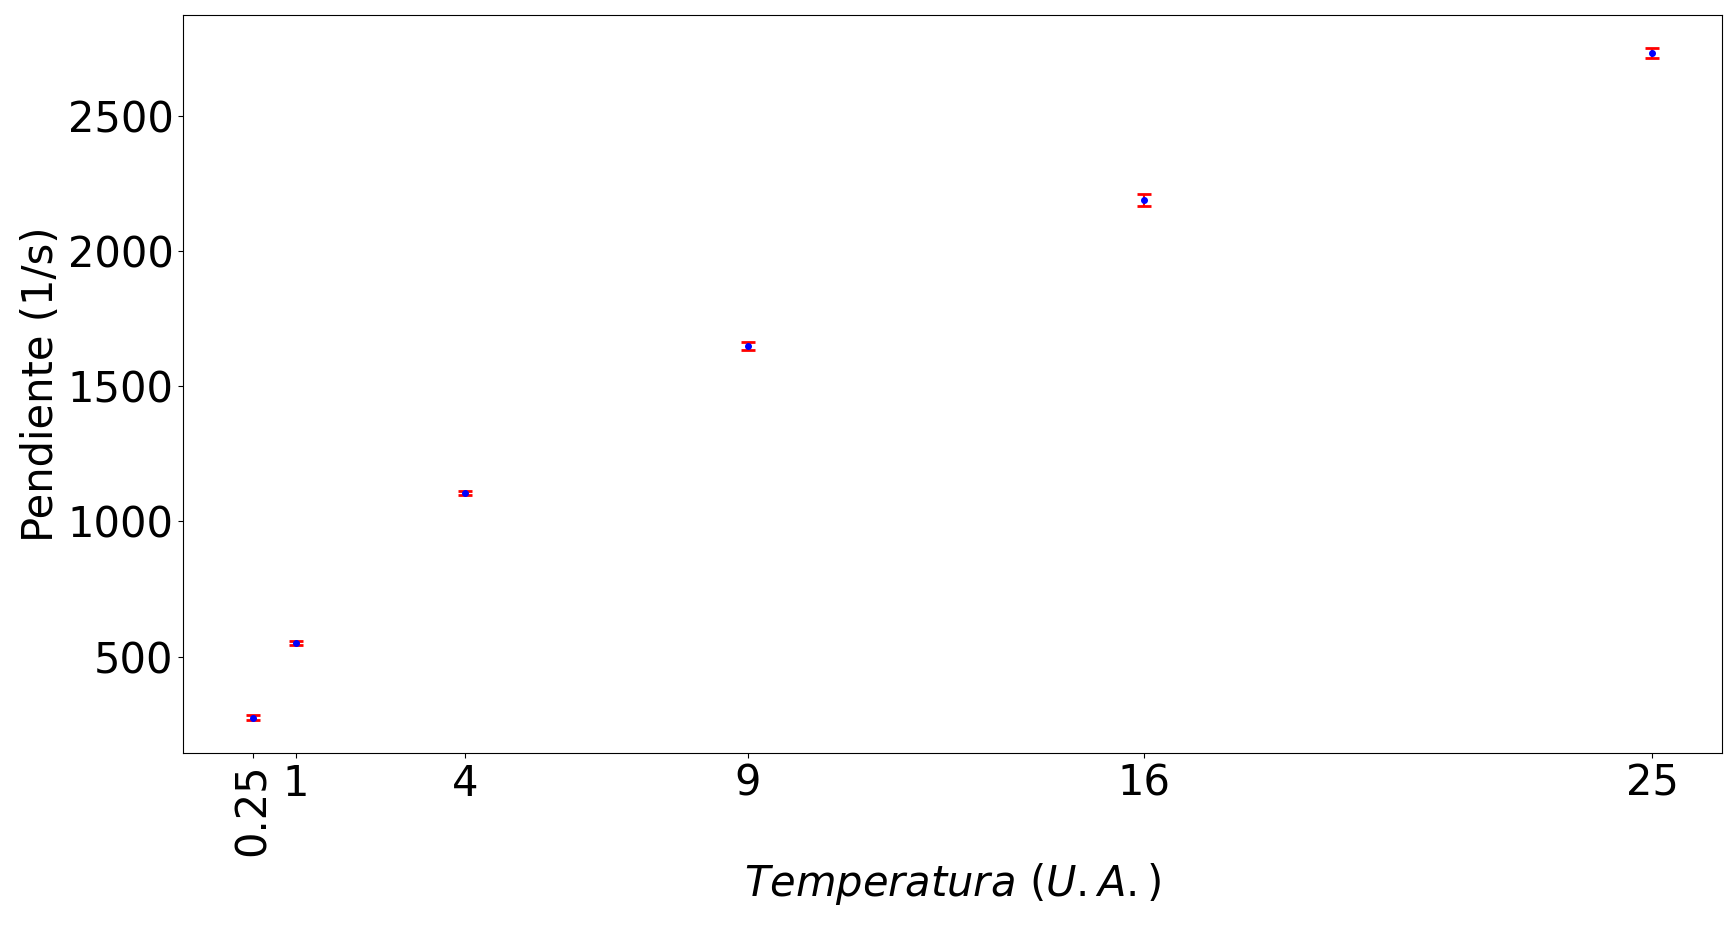
\includegraphics[width=0.6\textwidth]{pic/ejer3/bObs}
        \label{fig:ejer3:bobservable}
    \end{figure}

\end{frame}


\begin{frame}{Partícula grande libre}
    \begin{minipage}{0.45\textwidth}
        \begin{block}{Parámetros variables}
            \begin{itemize}
                \item $v_0 = 1\ m/s$
                \item $N = 300$
                \item $I = 20$
                \item $T = 1.5\ s$
            \end{itemize}
        \end{block}
    \end{minipage}
    \hfill
    \begin{minipage}{0.45\textwidth}
        \begin{figure}[H]
            \centering
            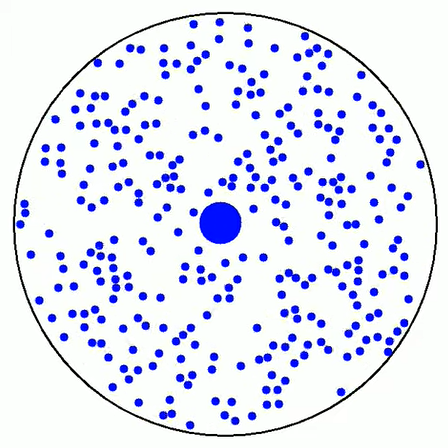
\includegraphics[width=0.8\textwidth]{pic/05-results/dcm_animation}
            \label{fig:dcm-animation}
        \end{figure}
        \tiny{\href{https://youtube.com/shorts/20RzmrMseC0?feature=share}{https://youtube.com/shorts/20RzmrMseC0?feature=share}}
    \end{minipage}
\end{frame}

\begin{frame}{Partícula grande libre}
    \textbf{Desplazamiento cuadrático medio}
    \begin{minipage}[c]{0.8\linewidth}
        \begin{figure}[H]
            \centering
            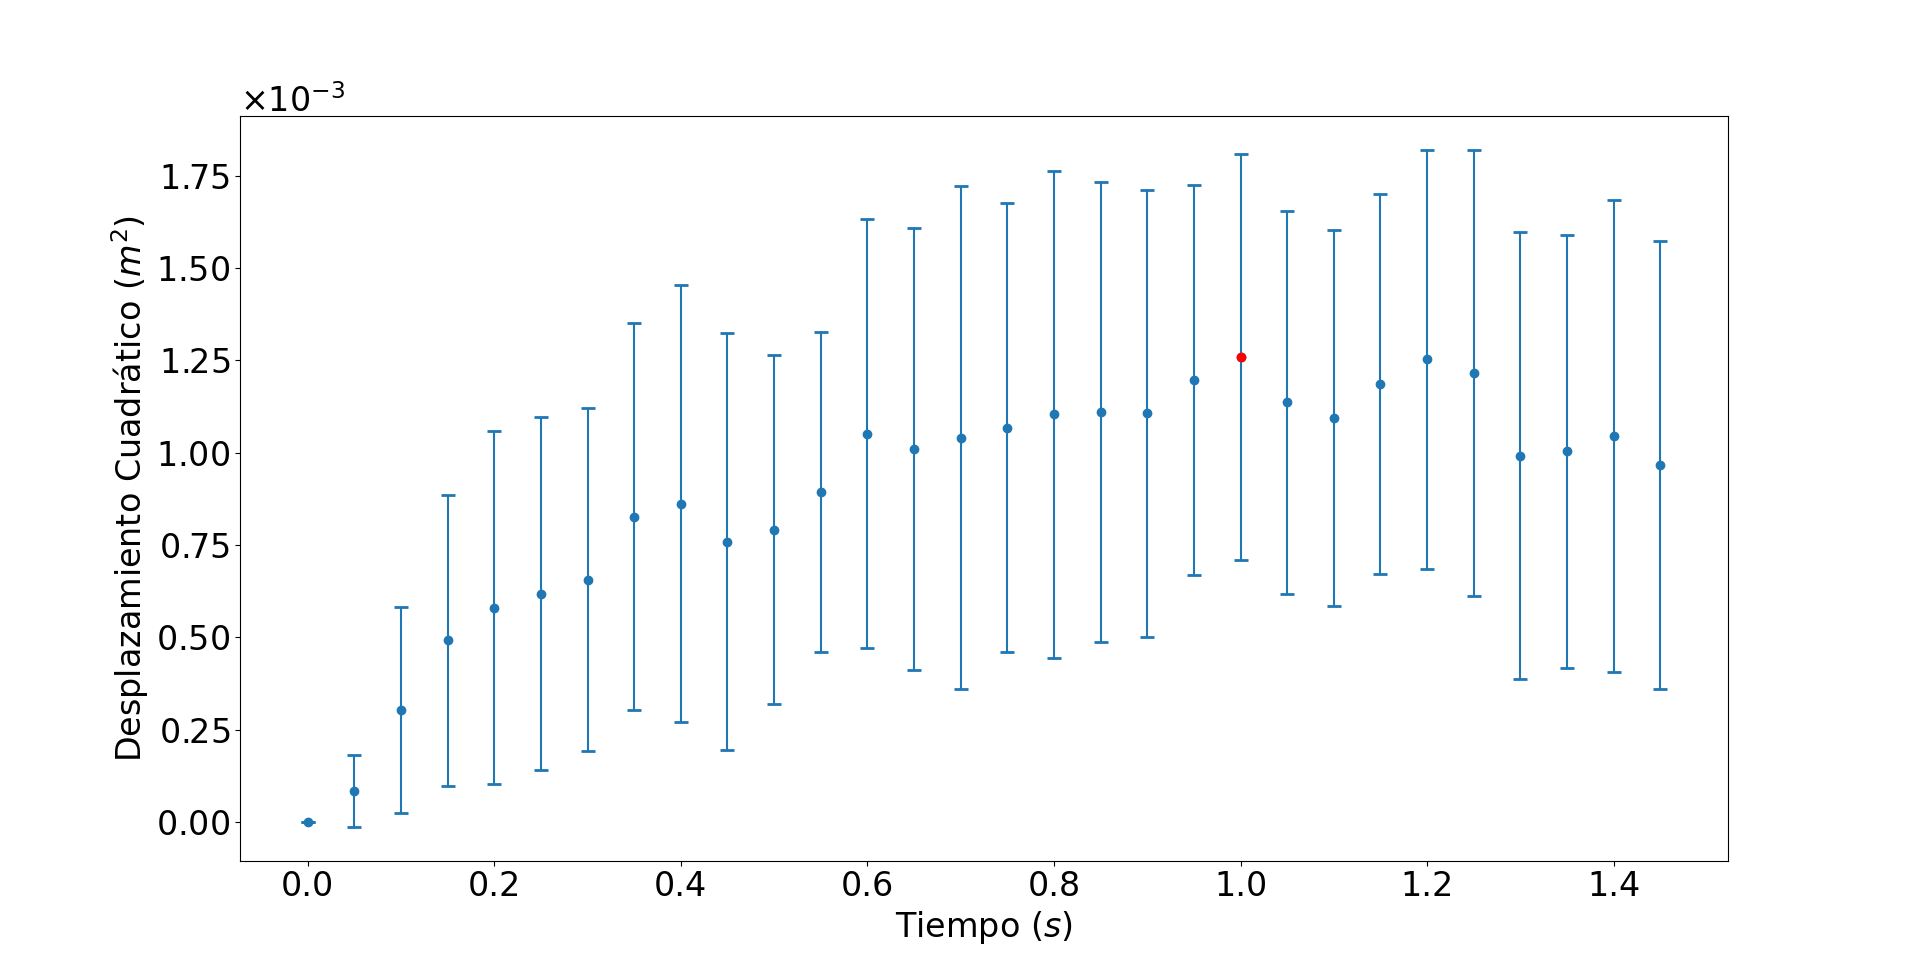
\includegraphics[width=0.9\textwidth]{pic/05-results/dcm_graph}
            \label{fig:dcm-graph}
        \end{figure}
    \end{minipage}
    \begin{minipage}[c]{0.15\linewidth}
        \text{$\Delta{t} = 0.05s$}
    \end{minipage}
\end{frame}

\begin{frame}{Partícula grande libre}
    \textbf{Ajuste lineal del coeficiente de difusión $D$}
    \begin{minipage}[c]{0.8\linewidth}
        \begin{figure}[H]
            \centering
            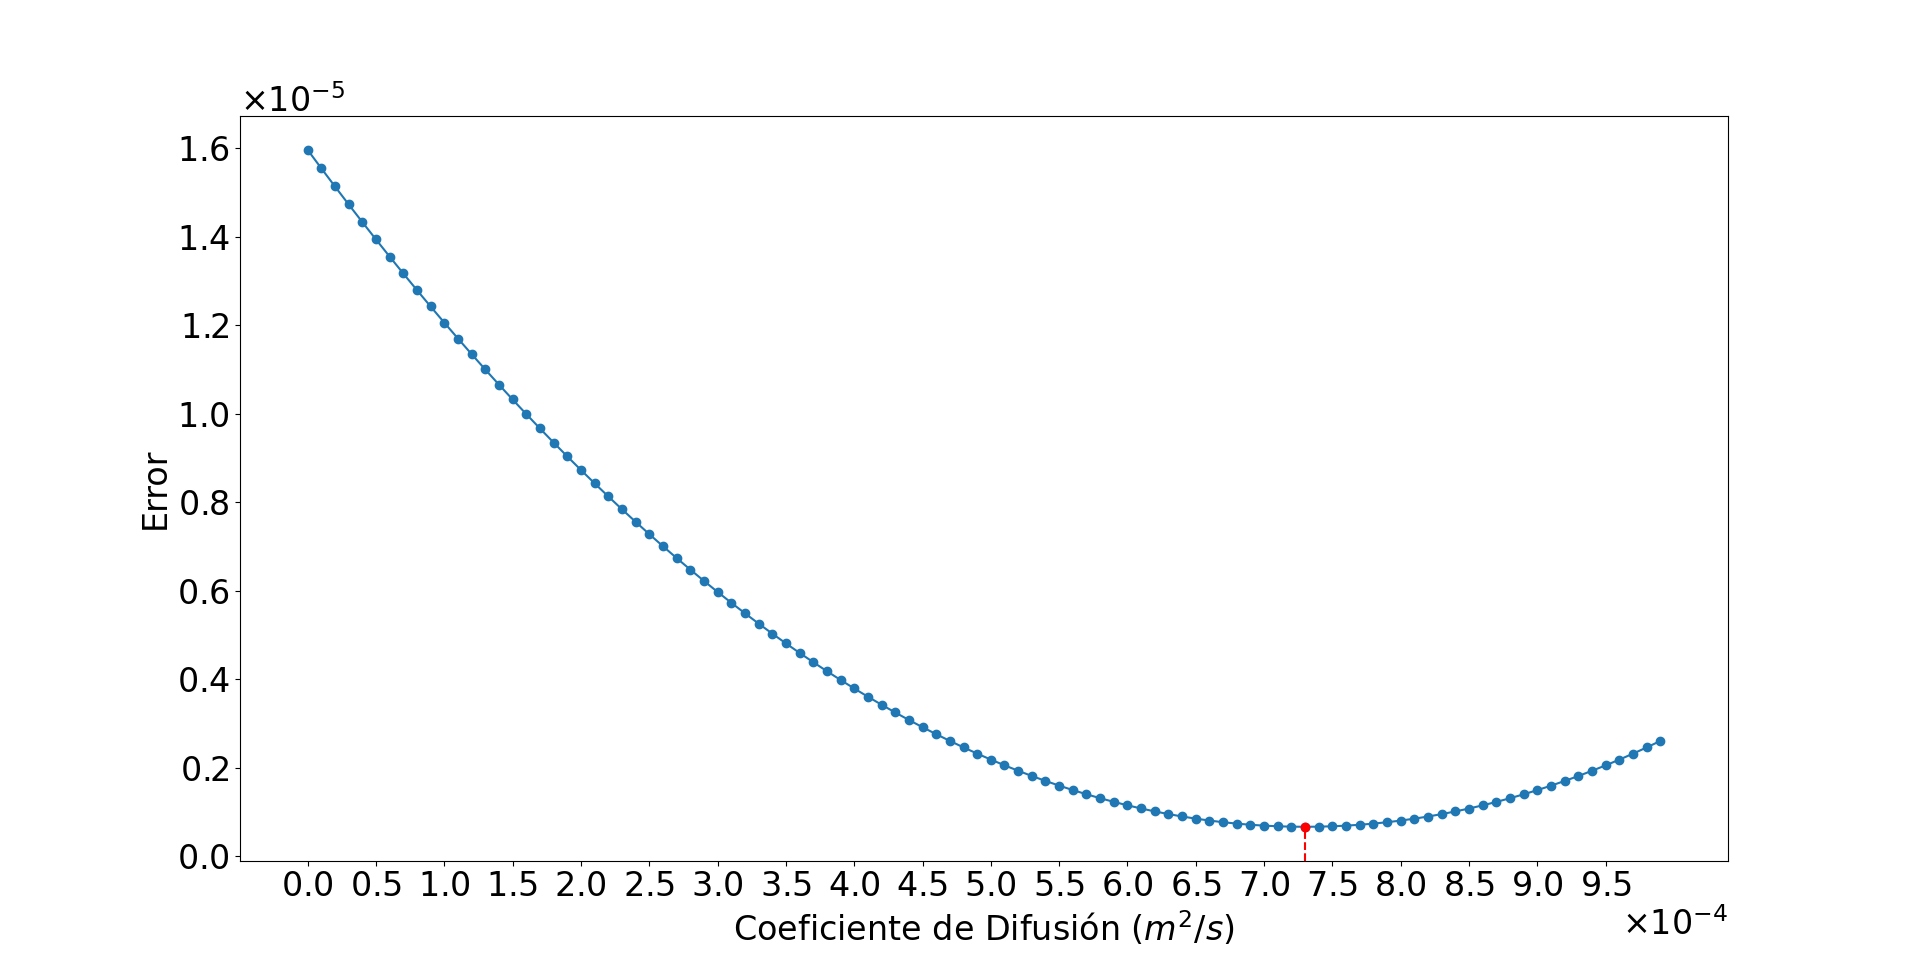
\includegraphics[width=0.9\textwidth]{pic/05-results/dcm_slope}
            \label{fig:dcm-slope}
        \end{figure}
    \end{minipage}
    \begin{minipage}[c]{0.15\linewidth}
        \text{$D = 7.3*10^{-4} \frac{m^{2}}{s}$}
    \end{minipage}
\end{frame}

\begin{frame}{Partícula grande libre}
    \textbf{Desplazamiento cuadrático medio}
    \begin{figure}[H]
        \centering
        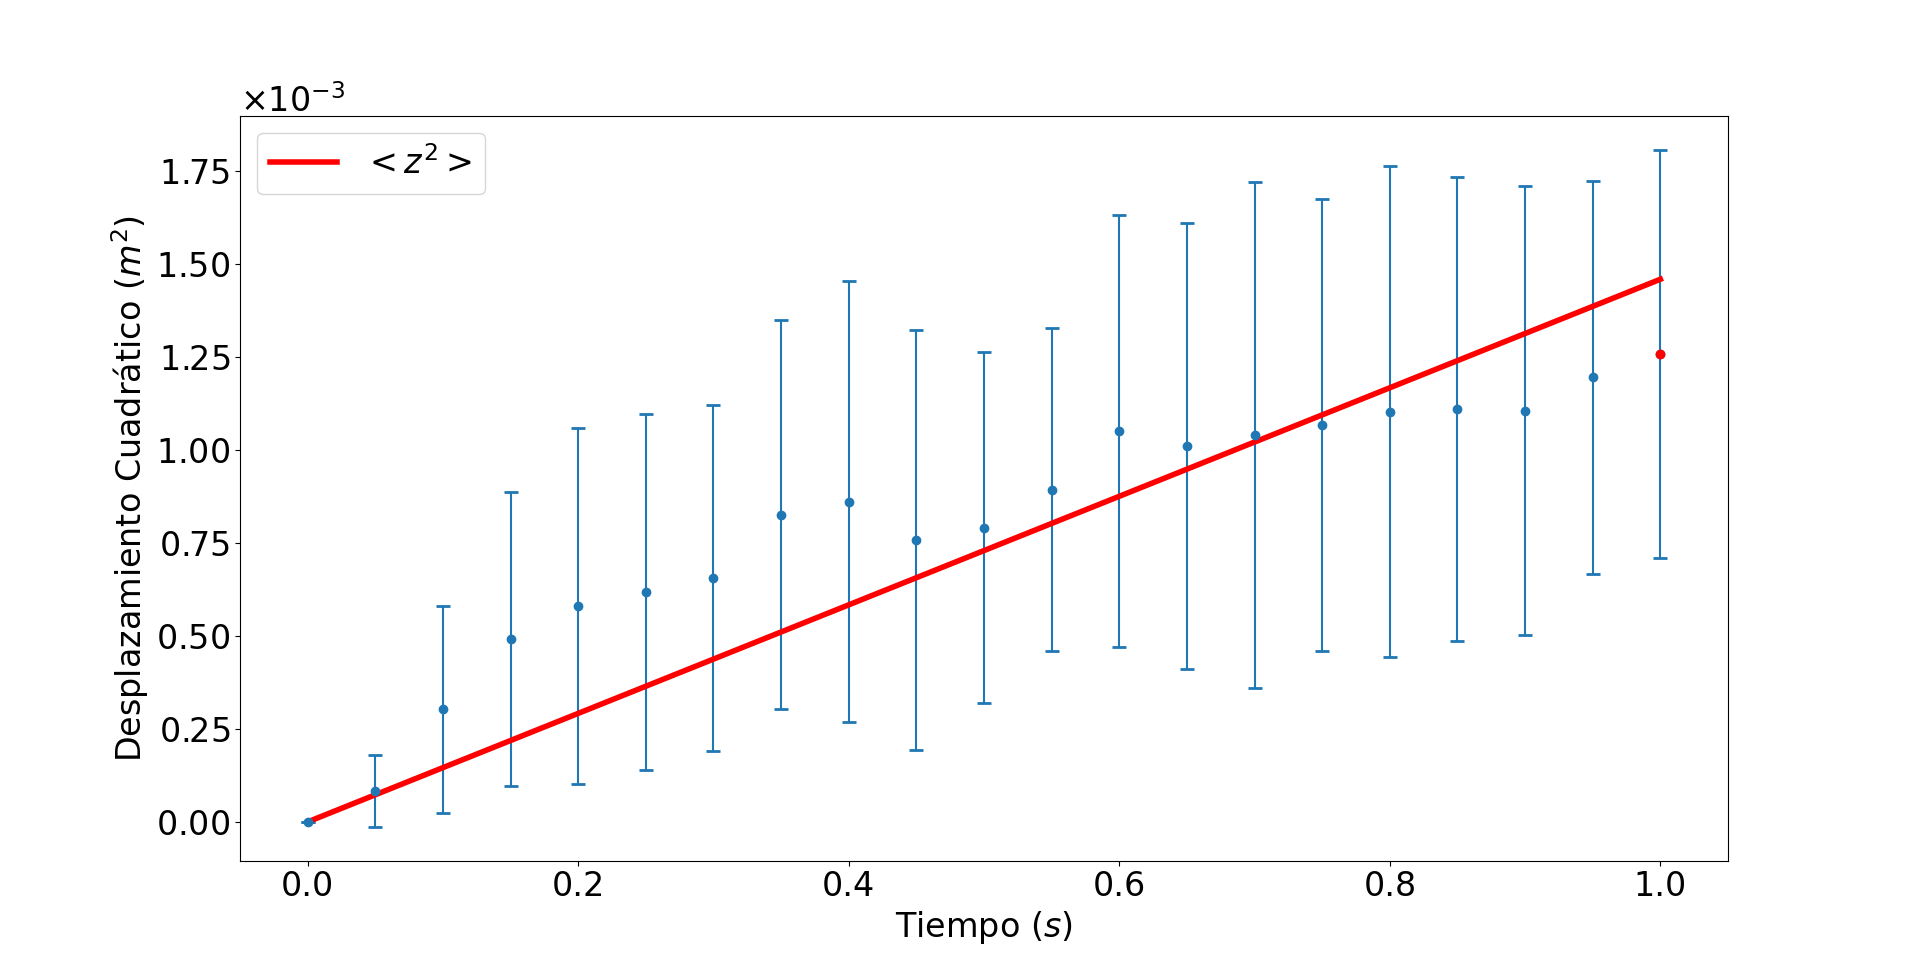
\includegraphics[width=0.9\textwidth]{pic/05-results/dcm_graph_and_slope}
        \label{fig:dcm-graph-and-slope}
    \end{figure}
\end{frame}


